\documentclass{article}
\usepackage[utf8]{inputenc}
\usepackage[T5]{fontenc}
\usepackage{graphicx}
\usepackage[margin=2cm]{geometry}
\title{Report 10: Kuwahara Filter}
\author{Nguyễn Thanh Hùng -- 2540056}
\date{October 8, 2026}

\begin{document}
\maketitle

\section{Implementation}
I first calculated HSV brightness $V=\max(R,G,B)/255$. For each pixel, the Kuwahara filter compares four $3\times3$ windows and selects the RGB mean of the window with the smallest V variance. The radius is 2 and the two-pixel border is preserved. The shared-memory version loads a $20\times20$ RGB/V tile, including its halo, for a $16\times16$ block and synchronizes before filtering.

I ran the notebook on Google Colab with a Tesla T4 and a $256\times256$ sample image.
GPU timings use \texttt{time.time()} after warm-up and synchronization, averaged over three runs; allocation and image transfers are excluded. Where measured, CPU time is one run; speedup is relative to that Python CPU implementation.

\section{Results}
CPU filter time: 6720.2551 ms. RGB-to-HSV time: 0.1260 ms (measured separately). Maximum pixel error: 0.
\begin{center}
\begin{tabular}{lrr}
\hline
Filter & GPU (ms) & CPU/GPU speedup \\
\hline
Global & 0.8864 & 7581.2 \\
Shared & 0.9138 & 7354.4 \\
\hline
\end{tabular}
\end{center}\begin{center}
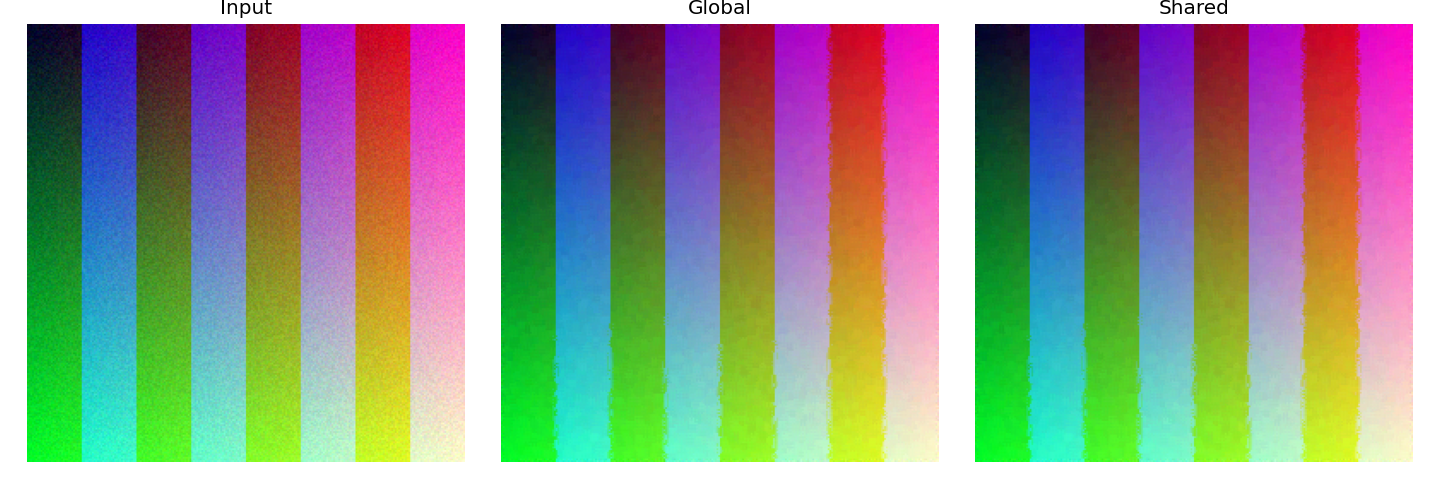
\includegraphics[width=.85\linewidth,height=.19\textheight,keepaspectratio]{figures/images.png}
\end{center}
\begin{center}
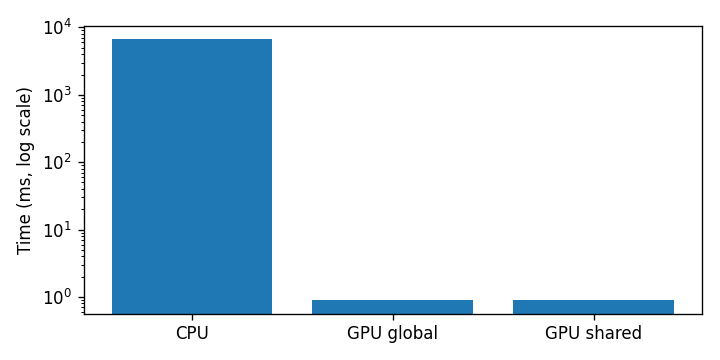
\includegraphics[width=.65\linewidth,height=.17\textheight,keepaspectratio]{figures/performance.png}
\end{center}

\section{Discussion}
The global/shared time ratio was 0.9701, so the shared version was about 3.1\% slower. Shared tiles reuse neighborhoods, while adjacent x threads access adjacent pixels. Tile loading and synchronization can add overhead. I did not profile bank conflicts.

\end{document}
